% P08-F03 universal preprocessing renderer output -- copied estimates only
%% source SHA256: 8c910290a3d09cbc9f03e7dcde77ae1598487533b0c68cfa1709a42e7d38621d
%% semantic SHA256: 7045e1dc2788300144330414456a5725a0e4cd3af23681b05b2c9e546cf3b73c
\documentclass[border=0pt]{standalone}
\usepackage[T1]{fontenc}
\usepackage[utf8]{inputenc}
\usepackage{lmodern}
\usepackage{tikz}
\usepackage{pgfplots}
\pgfplotsset{compat=1.18}
\definecolor{PolA}{HTML}{0072B2}
\pgfplotsset{pt0/.style={only marks, mark=*, color=PolA, mark options={fill=PolA, draw=black}}}
\pgfplotsset{bar0/.style={PolA, line width=0.8pt, mark=|, mark options={color=PolA}}}
\definecolor{PolB}{HTML}{D55E00}
\pgfplotsset{pt1/.style={only marks, mark=square*, color=PolB, mark options={fill=PolB, draw=black}}}
\pgfplotsset{bar1/.style={PolB, line width=0.8pt, mark=|, mark options={color=PolB}}}
\pgfplotsset{domainpts/.style={only marks, mark=o, mark options={draw=gray, fill=none, scale=0.7}}}
\tikzset{intervalna/.style={font=\fontsize{8}{10}\selectfont, anchor=east}}
\begin{document}
\begin{minipage}{181.86mm}\centering
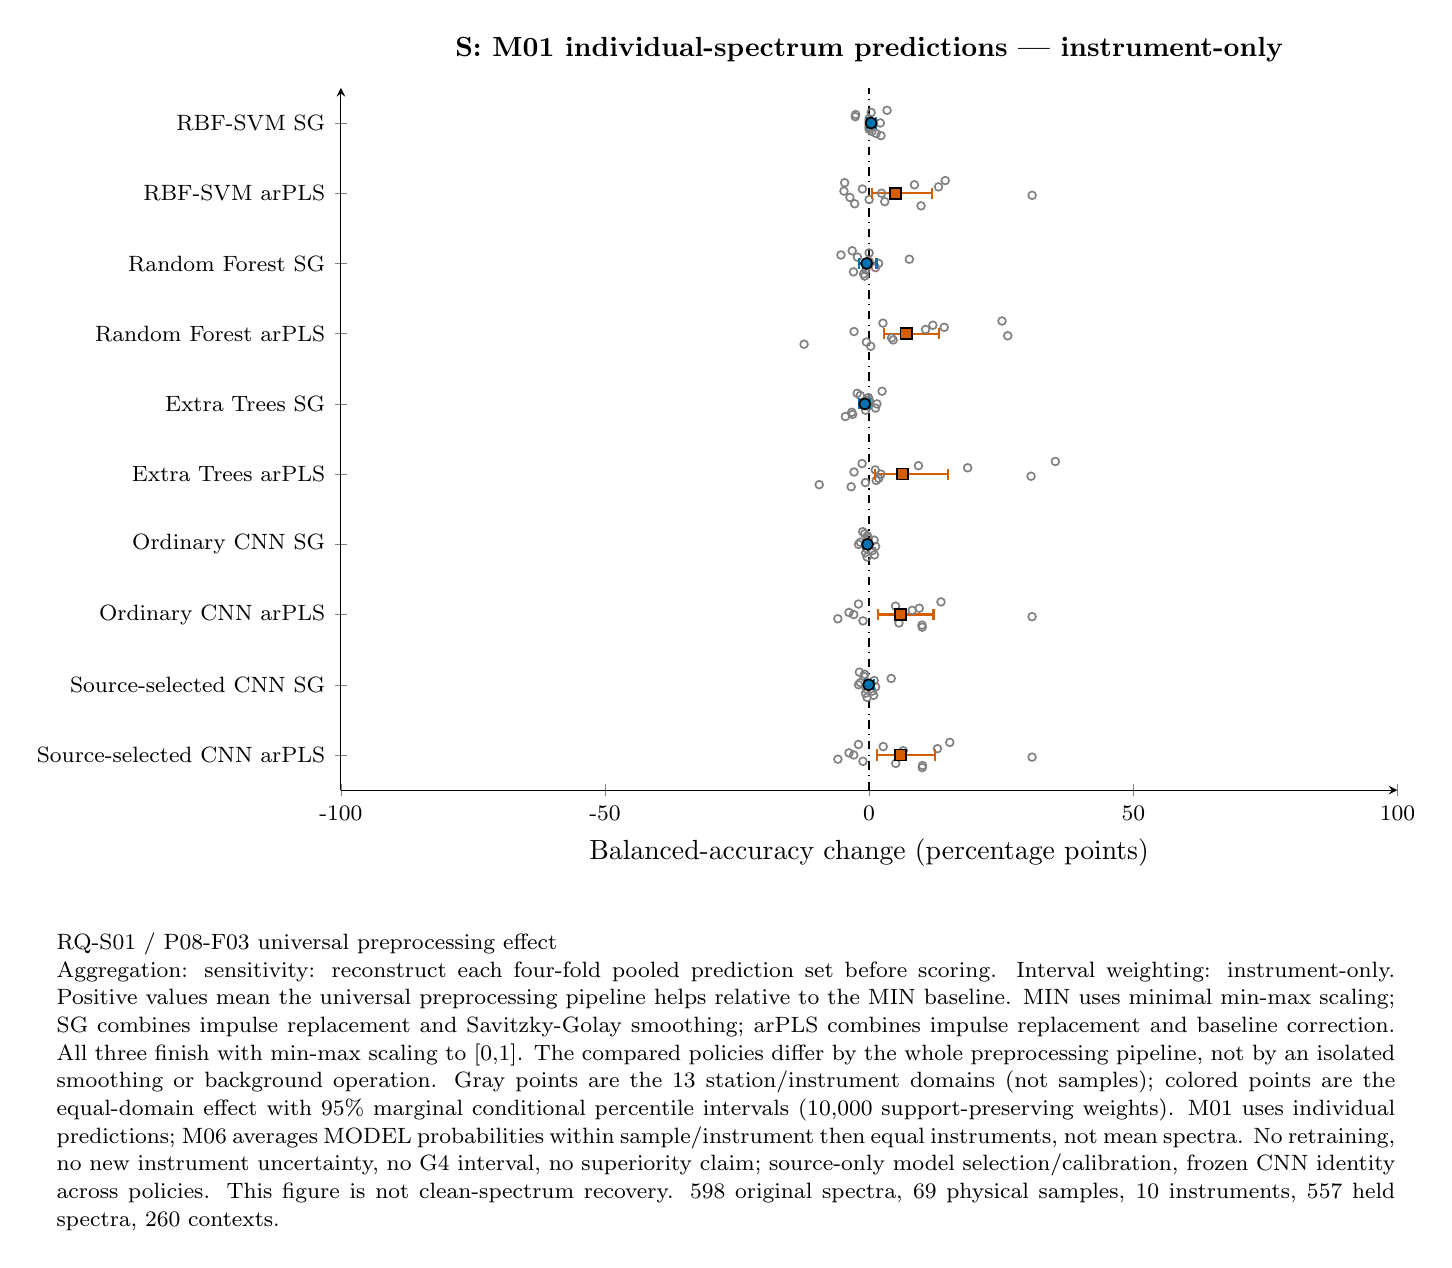
\begin{tikzpicture}
\begin{axis}[width=150mm, height=105mm, clip=false, xmin=-1, xmax=1, xtick={-1,-0.5,0,0.5,1}, xticklabels={-100,-50,0,50,100}, xlabel={Balanced-accuracy change (percentage points)}, ymin=-0.5, ymax=9.5, ytick={0,1,2,3,4,5,6,7,8,9}, yticklabels={{Source-selected CNN arPLS}, {Source-selected CNN SG}, {Ordinary CNN arPLS}, {Ordinary CNN SG}, {Extra Trees arPLS}, {Extra Trees SG}, {Random Forest arPLS}, {Random Forest SG}, {RBF-SVM arPLS}, {RBF-SVM SG}}, yticklabel style={font=\fontsize{8}{10}\selectfont}, tick label style={font=\fontsize{8}{10}\selectfont}, axis lines=left, title={S: M01 individual-spectrum predictions | instrument-only}, title style={font=\bfseries\fontsize{10}{12}\selectfont}, every axis plot/.append style={line width=0.6pt}]
\draw[black, dash dot, line width=0.6pt] (axis cs:0,-0.5) -- (axis cs:0,9.5);
\addplot[domainpts] coordinates {(0.022460317460317458,8.8200000000000003) (0.013248677248677249,8.8499999999999996) (0.005333333333333334,8.8800000000000008) (0,8.9100000000000001) (0,8.9399999999999995) (0,8.9700000000000006) (0.021164021164021163,9) (0,9.0299999999999994) (0,9.0600000000000005) (-0.026262626262626258,9.0899999999999999) (-0.025454545454545459,9.1199999999999992) (0.0038095238095238104,9.1500000000000004) (0.03390804597701149,9.1799999999999997)};
\addplot[bar0] coordinates {(-0.0038611013935407278,9) (0.012473496213407374,9)};
\addplot[pt0] coordinates {(0.0037082113289009836,9)};
\addplot[domainpts] coordinates {(0.09825396825396826,7.8200000000000003) (-0.027343915343915344,7.8499999999999996) (0.029575757575757578,7.8799999999999999) (0,7.9100000000000001) (-0.036363636363636362,7.9400000000000004) (0.30854838709677412,7.9699999999999998) (0.023544973544973542,8) (-0.047619047619047616,8.0299999999999994) (-0.012698412698412691,8.0600000000000005) (0.1313131313131313,8.0899999999999999) (0.085757575757575741,8.1199999999999992) (-0.046349206349206348,8.1500000000000004) (0.14406130268199233,8.1799999999999997)};
\addplot[bar1] coordinates {(0.00480017224407823,8) (0.11904107488590432,8)};
\addplot[pt1] coordinates {(0.050052375219227271,8)};
\addplot[domainpts] coordinates {(-0.0083333333333333332,6.8200000000000003) (-0.010433862433862431,6.8499999999999996) (-0.029575757575757578,6.8799999999999999) (-0.0060606060606060606,6.9100000000000001) (0.012121212121212121,6.9400000000000004) (-0.005333333333333334,6.9699999999999998) (0.017923280423280421,7) (0,7.0300000000000002) (0.076190476190476183,7.0599999999999996) (-0.02222222222222222,7.0899999999999999) (-0.05333333333333333,7.1200000000000001) (0,7.1500000000000004) (-0.031992337164750959,7.1799999999999997)};
\addplot[bar0] coordinates {(-0.019447681794047562,7) (0.013864731591881913,7)};
\addplot[pt0] coordinates {(-0.0046961397478638856,7)};
\addplot[domainpts] coordinates {(0.00301587301587301,5.8200000000000003) (-0.1231111111111111,5.8499999999999996) (-0.0050909090909090895,5.8799999999999999) (0.045454545454545456,5.9100000000000001) (0.042424242424242427,5.9400000000000004) (0.26237096774193552,5.9699999999999998) (0.066798941798941788,6) (-0.028571428571428571,6.0300000000000002) (0.10687830687830688,6.0599999999999996) (0.1420875420875421,6.0899999999999999) (0.12060606060606061,6.1200000000000001) (0.026190476190476188,6.1500000000000004) (0.25153256704980842,6.1799999999999997)};
\addplot[bar1] coordinates {(0.027655593137028218,6) (0.13215003986104237,6)};
\addplot[pt1] coordinates {(0.070045082651867971,6)};
\addplot[domainpts] coordinates {(-0.044999999999999998,4.8200000000000003) (-0.031153439153439148,4.8499999999999996) (-0.032969696969696968,4.8799999999999999) (-0.0066666666666666662,4.9100000000000001) (0.012121212121212121,4.9400000000000004) (-0.002666666666666667,4.9699999999999998) (0.014814814814814814,5) (0,5.0300000000000002) (0,5.0599999999999996) (-0.0013468013468013462,5.0899999999999999) (-0.016666666666666666,5.1200000000000001) (-0.022619047619047618,5.1500000000000004) (0.024521072796934863,5.1799999999999997)};
\addplot[bar0] coordinates {(-0.019243535671812178,5) (0.0022415694949075105,5)};
\addplot[pt0] coordinates {(-0.0082793757966171753,5)};
\addplot[domainpts] coordinates {(-0.033968253968253974,3.8199999999999998) (-0.094455026455026458,3.8500000000000001) (-0.0070303030303030308,3.8799999999999999) (0.013333333333333332,3.9100000000000001) (0.018181818181818181,3.9399999999999999) (0.30646236559139789,3.9700000000000002) (0.022354497354497356,4) (-0.028571428571428571,4.0300000000000002) (0.01164021164021164,4.0599999999999996) (0.18653198653198649,4.0899999999999999) (0.093333333333333324,4.1200000000000001) (-0.013412698412698414,4.1500000000000004) (0.35249042145593867,4.1799999999999997)};
\addplot[bar1] coordinates {(0.010888055448490199,4) (0.14945006854144788,4)};
\addplot[pt1] coordinates {(0.063606942844985109,4)};
\addplot[domainpts] coordinates {(-0.0038095238095238078,2.8199999999999998) (0.010095238095238096,2.8500000000000001) (-0.0067878787878787889,2.8799999999999999) (0.0060606060606060606,2.9100000000000001) (-0.0051282051282051291,2.9399999999999999) (0.012301075268817204,2.9700000000000002) (-0.020039682539682541,3) (-0.01666666666666667,3.0299999999999998) (0.0095238095238095229,3.0600000000000001) (-0.0013468013468013462,3.0899999999999999) (-0.0033333333333333331,3.1200000000000001) (-0.0083333333333333332,3.1499999999999999) (-0.012068965517241379,3.1800000000000002)};
\addplot[bar0] coordinates {(-0.0085761200930682888,3) (0.0017746854672717799,3)};
\addplot[pt0] coordinates {(-0.0030410508857073421,3)};
\addplot[domainpts] coordinates {(0.10055555555555555,1.8200000000000001) (0.10004232804232804,1.8500000000000001) (0.056484848484848492,1.8799999999999999) (-0.011666666666666667,1.9099999999999999) (-0.059207459207459213,1.9399999999999999) (0.30840860215053761,1.97) (-0.029100529100529106,2) (-0.038095238095238092,2.0299999999999998) (0.081481481481481474,2.0600000000000001) (0.094949494949494936,2.0899999999999999) (0.049999999999999996,2.1200000000000001) (-0.020238095238095239,2.1499999999999999) (0.13601532567049807,2.1800000000000002)};
\addplot[bar1] coordinates {(0.016386922918355008,2) (0.12165355619508469,2)};
\addplot[pt1] coordinates {(0.059202280617442753,2)};
\addplot[domainpts] coordinates {(-0.0038095238095238078,0.82000000000000006) (0.008486772486772487,0.84999999999999998) (-0.0067878787878787889,0.88) (0.0060606060606060606,0.91000000000000003) (-0.0051282051282051291,0.93999999999999995) (0.012301075268817204,0.96999999999999997) (-0.020039682539682541,1) (-0.01666666666666667,1.03) (0.0095238095238095229,1.0600000000000001) (0.041750841750841747,1.0900000000000001) (-0.01,1.1200000000000001) (-0.0083333333333333332,1.1499999999999999) (-0.018486590038314175,1.1799999999999999)};
\addplot[bar0] coordinates {(-0.0081147333702803991,1) (0.0091370605026769459,1)};
\addplot[pt0] coordinates {(-0.00085605963175057107,1)};
\addplot[domainpts] coordinates {(0.10055555555555555,-0.17999999999999999) (0.10107936507936507,-0.14999999999999999) (0.050424242424242427,-0.12) (-0.011666666666666667,-0.089999999999999997) (-0.059207459207459213,-0.059999999999999998) (0.30840860215053761,-0.029999999999999999) (-0.029100529100529106,0) (-0.038095238095238092,0.029999999999999999) (0.064550264550264552,0.059999999999999998) (0.12929292929292929,0.089999999999999997) (0.026666666666666665,0.12) (-0.020238095238095239,0.14999999999999999) (0.15268199233716476,0.17999999999999999)};
\addplot[bar1] coordinates {(0.015622395204672835,0) (0.12489757014662668,0)};
\addplot[pt1] coordinates {(0.059642433057595201,0)};
\end{axis}
\node[anchor=north, align=justify, text width=170mm, font=\fontsize{8}{10}\selectfont] at ([yshift=-6mm]current bounding box.south) {RQ-S01 / P08-F03 universal preprocessing effect\\ Aggregation: sensitivity: reconstruct each four-fold pooled prediction set before scoring. Interval weighting: instrument-only. Positive values mean the universal preprocessing pipeline helps relative to the MIN baseline. MIN uses minimal min-max scaling; SG combines impulse replacement and Savitzky-Golay smoothing; arPLS combines impulse replacement and baseline correction. All three finish with min-max scaling to [0,1]. The compared policies differ by the whole preprocessing pipeline, not by an isolated smoothing or background operation. Gray points are the 13 station/instrument domains (not samples); colored points are the equal-domain effect with 95\% marginal conditional percentile intervals (10,000 support-preserving weights). M01 uses individual predictions; M06 averages MODEL probabilities within sample/instrument then equal instruments, not mean spectra. No retraining, no new instrument uncertainty, no G4 interval, no superiority claim; source-only model selection/calibration, frozen CNN identity across policies. This figure is not clean-spectrum recovery. 598 original spectra, 69 physical samples, 10 instruments, 557 held spectra, 260 contexts.};
\end{tikzpicture}
\end{minipage}
\end{document}
